\documentclass[AMA,STIX1COL]{WileyNJD-v2}

\articletype{Article Type}%

\received{01 June 2018}
\revised{01 August 2018}
\accepted{01 August 2018}

\raggedbottom
\usepackage{subcaption}
\captionsetup[subfigure]{font=normalsize}

\usepackage{glossaries}
\makeglossaries

\begin{document}

\title{Open-source platforms for fast room acoustic simulations in complex structures}
%\title{This is the sample article title\protect\thanks{This is an example for title footnote.}}

\author[1]{Matthieu Aussal}

\author[2]{Robin Gueguen}



%\author[3]{Author Three}

\authormark{AUSSAL \& GUEGUEN}

\address[1]{\orgdiv{Centre de math\'ematique appliqu\'ees}, \orgname{\'Ecole Polytechnique}, \orgaddress{91128 Palaiseau, \country{France}}}

\address[2]{\orgdiv{Institut des Sciences du Calcul et des Donn\'ees}, \orgname{Sorbonne Universit\'e}, \orgaddress{Campus Pierre et Marie Curie - 4 place Jussieu, 75252 Paris Cedex 05 \country{France}}}




\corres{ \email{matthieu.aussal@polytechnique.edu}\\\email{gueguen.robin@gmail.com}}

%\presentaddress{This is sample for present address text this is sample for present address text}

\abstract[Summary]{
This article presents new numerical simulation tools, both for Matlab and Blender CAD software. Available in open-source under GPL 3.0 license, it uses a ray tracing / image-sources hybrid method to calculate room acoustics for large meshes. Performances are optimized to solve significant size numerical problems (typically more than 100,000 surface elements and about a million of \textit{rays}). For this purpose, a \textit{Divide and Conquer} approach with a recursive octree structure has been implemented to reduce the quadratic complexity of the ray/element interactions to near-linear. Thus, execution times are less sensitive to mesh density, which allows complex geometry simulations. After ray propagation, a hybrid method leads to image-sources format, which can be visually analyzed to localize sound map. Finally, impulse responses are constructed from the image-sources and FIR filters are proposed natively over 8 octave bands, taking into account material absorption properties and propagation medium. This algorithm is validated by various comparison with theoretical test cases. Furthermore, an exemple on a complex case with the ancient theater of Orange is presented. 
}

\keywords{room acoustic, ray-tracing, image-sources, octree, Matlab, Blender, archeology, open-source}

\jnlcitation{\cname{%
\author{M. Aussal}, and
\author{R. Gueguen}, 
} (\cyear{2018}), 
\ctitle{Room acoustic measurement tool for complex geometry}, \cjournal{International Journal for Numerical Methods in Engineering}, \cvol{2018;00:1--6}.}

\maketitle

%\footnotetext{\textbf{Abbreviations:} ANA, anti-nuclear antibodies; APC, antigen-presenting cells; IRF, interferon regulatory factor}

% glossaire
%\section{Glossary\label{app1}}
%\newacronym{CAD}{CAD}{Computer-Aided Design}
%\newacronym{rir}{RIR}{\emph{Room Impulse response}}
%\newacronym{RT60}{$RT_{60}$}{\emph{Reveberation Time at $-60dB$}}
%\newacronym{orchestra}{\textit{orchestra}}{\emph{Semicircular (Roman) or circular (Greek) space between the stage and the first tier}}
%
%\gls{CAD}\\
%\gls{rir}\\
%\gls{RT60}\\
%\gls{orchestra} 

\section*{Introduction}
\label{sec1}
Today, digital technologies allow research to explore previously inaccessible areas, as virtual reality for archaeology. In this domain, many works focus on the visual restitution, but acoustic studies can reinforce researches to improve the understanding of the ancient world. For example, during the Roman Empire, architects have designed buildings also based on the sound propagation they wanted to achieve\cite{vitruve}. In this study, we focus on the ancient theater of Orange which has a significant size (100m wide), a complex geometry (decoration, gradins, colonnes, arcades ...) and which is open air. In a previous work, a complete mesh was designed using Blender CAD software (citer Blender), according to the most recent archeological knowledge \cite{theseRobin}. To be representative, this mesh has hundreds of thousands of elements (triangular faces), with complex shape (inserer figure maillage pour montrer la complexite). As this numerical model is now used by researchers to perform archeological hypothesis, we developed our own room acoustic software, directly integrated in the archeologists workflow. As the mesh size makes difficult the use of precise methods (FEM, BEM, ...), this software is based on a ray-tracing approximation, in order to compute fastly the full-band room impulse response (50 to 15000Hz). This tool has been developed following two steps. We first build a prototype using Gypsilab, an open source Matlab framework for fast prototyping (citer le papier gypsilab). This preliminary work was usefull to construct and validate ideas and algorithms. It conducts to the creation of a new toolbox, now added to the master branch of Gypsilab, and freely downloadable (citer adresse github). In a second step, all algorithms was retranscrypted in C++ using Qt Creator, leading to an autonomous library. A python interface was added, in order to use this library as a Blender plug'in. At the end, this plug'in allow archeologists to only work on Blender, modifying easily meshes and materials, run acoustic simulation and visualize results. \\
After reminders on acoustical energy propagation represented by ray-tracing, this paper gives implementation details for fast computation for large meshes. At the end, validation test cases are given and application on our modelization of the ancient theater of Orange is performed. 




\section{Acoustical energy modelization}\label{sec2}
\subsection{Continuous domain equation}

By modelling a point sound source as a localized pulse in space, the associated acoustical energy E(t) propagates \cite{jouhaneau} over time on a spherical surface $S(t)$, such that :
%
\begin{equation} 
E(t) = E_0 \int_{S(t)} \overrightarrow{I}(t).\overrightarrow{ds} \qquad \forall t > 0,
\end{equation}
%
with $E_0$ the initial energy and $\overrightarrow{I}(t)$ the acoustical intensity. According to the first principle of thermodynamics and by neglecting the effects of losses related to the absorption of the propagation medium, the acoustic energy is preserved over time. Thus, for a normalized punctual source :
%
\begin{equation} 
\int_{S(t)} \overrightarrow{I}(t).\overrightarrow{ds} = 1 \qquad \forall t > 0.
\end{equation}
%
After integration on the spherical surface $S(t)$, the infinitesimal acoustic intensity is written :
\begin{align} 
% \overrightarrow{I}(t) &= \frac{ \overrightarrow{d}(t)}{4\pi d(t)^3} \qquad \forall t > 0 \nonumber, \\
|| \overrightarrow{I}(t) || &= \frac{1}{4\pi d(t)^2} \qquad \forall t > 0,
\end{align}
%
reflecting that intensity decreases as the square of the distance to the source d(t). Integrating on a portion $\sigma(t)$ of the complete sphere $S(t)$, the energy is then carried by the solid angle $\Omega_{\sigma}$ :
%
\begin{equation}
E_{\sigma}(t) = E_0 \int_{\sigma(t)}  \frac{1}{4\pi  d(t)^2} ds = \frac{E_0}{4\pi}  \Omega_{\sigma}.
\label{eq_4}
\end{equation}
%
This last equation shows that the energy of a solid angle is constant over time and corresponds to a portion of the initial energy~$E_0$. Thus, subdividing $S(t)$ in $N$ portions $\sigma_i(t)$, the total energy can be decomposed as a sum of elementary energies, carried by solid angles $\Omega_i$, such as : 
%
\begin{equation}
E(t) = \sum_{i=1}^N E_i(t) = \frac{E_0}{4\pi}  \sum_{i=1}^N \Omega_i  \qquad \forall t > 0.
\label{eq_5}
\end{equation}
Ones can notice that $(\Omega_i)_{i\in[1,N] }$ is a directional basis, representing energy propagation by piecewise constant elements. Furthermore, for greater clarity, we definitively set in the following $E_0 = 1$.

\subsection{Discrete model}

To numerically represent the energy propagation, we have to discretize basis $(\Omega_i)_{i\in[1,N] }$ in (eq.~\ref{eq_5}). For this purpose, we define a \textit{ray} object composed by :
\begin{itemize}
\item An origin coordinate $x_i$,
\item A direction vector $\overrightarrow{u_i}$,
\item An energy value $E_i$.
\end{itemize}

For example, with an omnidirectional source, \textit{rays} are given by :
\begin{itemize}
\item The source coordinate ($x_i = x_s,~\forall i\in[1,N]$),
\item A unit sphere uniform sampling (e.g.~icosahedre subdivision, Fibonacci's rule \cite{fibonacci}, etc.),
\item An uniform energy repartition ($E_i = \frac{4\pi}{N},~\forall i\in[1,N]$).
\end{itemize}

To complete this approach, we have to define a discrete measure of energy propagation. To this end, we consider a $r$-radius measurement sphere $S(x_m, r)$, centered on $x_m$.  We can then add the contributions of a $n$-\textit{rays}  beam that intersect this sphere to calculate the acoustic energy $E_m$ at point $x_m$ :

\begin{equation}
E_m \approx  \frac{1}{4\pi}  \sum_{i=1}^n E_i.
\end{equation}
In the particular case of an omnidirectionnal source, we have : 
\begin{equation}
E_m \approx  \frac{n}{N},
\end{equation}
which means that the measured energy $E_m$ is statistically represented by the ratio between the number of \textit{rays} forming a beam to the total number of \textit{rays}.

\begin{figure}[t]
\centering
	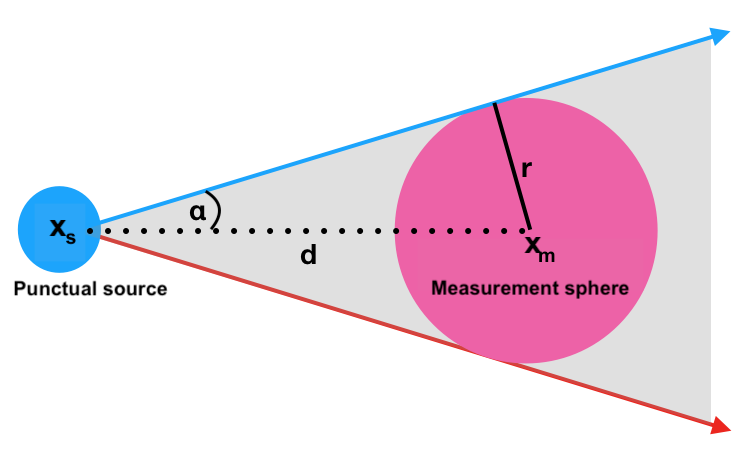
\includegraphics[width=0.6\linewidth]{schema_rayon}
	\caption{Representation of a $r$-radius measurement sphere centered in $x_m$, receiving energy from a sound source in $x_s$.}
	\label{schema_rayon}
\end{figure}

Moreover, applying the continuous model (eq.~\ref{eq_4}), the measured energy is given by :
\begin{equation}
E_m = \frac{1}{4\pi}  \Omega_m,
\end{equation}
where $\Omega_m$ is a solid angle of a cone of revolution (see fig. \ref{schema_rayon}), such as :
\begin{equation}
\Omega_m = 2\pi(1-\cos{\alpha}).
\end{equation}
Following the figure \ref{schema_rayon} :
\begin{equation}
\Omega_m = 2\pi \left( 1 - \sqrt{1-\frac{r^2}{d^2}} \right)
\end{equation}
and considering $\frac{r}{d} \ll 1$, 
\begin{equation}
\Omega_m = \pi \frac{r^2}{d^2}.
\end{equation}
At the end, 
\begin{equation}
E_m \approx  \frac{n}{N} \approx  \frac{\pi r^2}{4\pi d^2}.
\label{eq_12}
\end{equation}
To ensure the existence of this last approximation, beam has to be measurable and count at least one \textit{ray} ($n\geq1$). Thus, fixing a measurement radius r, approximation (\ref{eq_12}) gives a maximum validity range of the discrete model :  
\begin{equation}
\label{eq_13}
	d \leq \frac{r}{2}\sqrt{\frac{N}{n}}.
\end{equation}
In addition, figure \ref{energie} shows how this modelization fills with distance between source and measures. The accuracy of the measurement depends strongly on the number of  \textit{rays} counted, then, the more $n$ increases, the more accurate will be the measurement. Nevertheless, in practice, values for a short distance between the source and the measurement sphere represent direct sound and first reflections, whereas long distances describe the diffuse field. Under this assumption, we can consider this model acceptable for all beam such as $n\geq1$. 

\begin{figure}[t]
\centering
	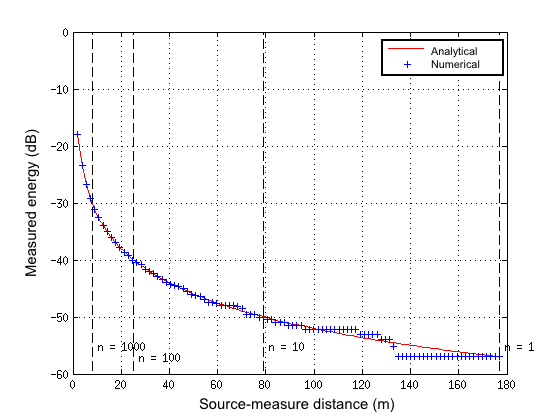
\includegraphics[width=0.8\linewidth]{energie.png}
	\caption{Measured energy (dB) in function of distance between $x_s$ and $x_m$ in meter for $r = 0.36$m and $N = 10^6$. Blue crosses stand for the statistical measure $f(r) = \frac{n(r)}{N}$ and red ligne the analytic function $f(r) = \frac{\pi r^2}{4\pi d^2}$.}
	\label{energie}
\end{figure}

%
\begin{figure}[t]
	\centering
	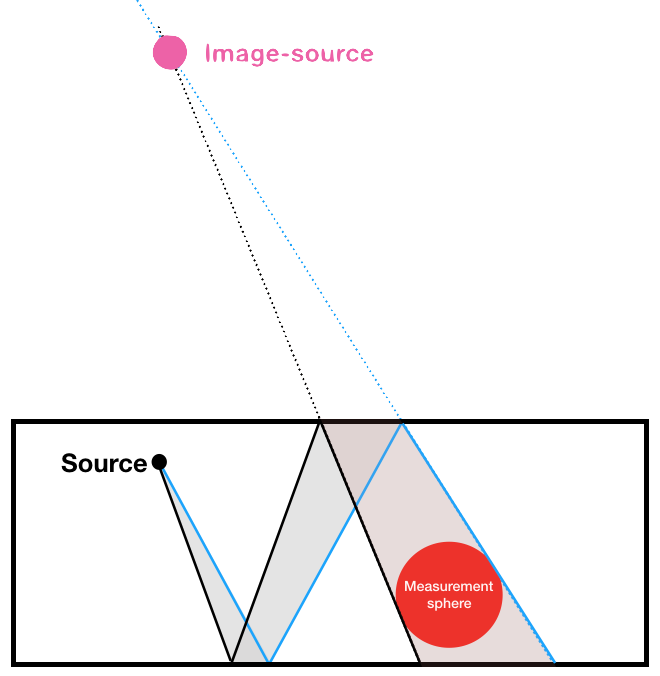
\includegraphics[width=0.7\linewidth]{schema_SI}
	\caption{Sketch of the creation of an image-source by successive reflections of a ray on the walls of a room.}
	\label{schema_SI}
\end{figure}
%Example for bibliography citations cite\cite{Taylor1937}, cites\cite{Knupp1999,Kamm2000}



\subsection{Presence of an obstacle}
For the case of acoustic propagation in presence of an obstacle, we choose to only consider specular reflections (Snell-Descartes laws). Indeed, this approximation is suitable when surfaces are large in comparaison to wavelengths, because diffraction effects can be neglected \cite{jouhaneau}. For a room, this condition is reached if :
\begin{equation}
ka \gg 1, 
\end{equation}
with $k$ the wave number and $a$ the characteristical diameter of the room \cite{hautes_freq}. This approach is currently used by room acoustic softwares (e.g. \textit{Odeon} \cite{odeon}, \textit{Grasshopper} \cite{grasshopper}, etc.) regarding to audible frequency range (62,5 to 15000Hz). In particular, as the Theater of Orange has a characteristical diameter about 50 meters, the high frequency approximation is reached. 

Following the discrete model, when an incident \textit{ray} collides a flat surface, a reflected \textit{ray} is generated from the collision point. Noting $\overrightarrow{u_i}$ the direction vector of the incident  \textit{ray}, the reflected direction vector $\overrightarrow{u_r}$ is defined by :
\begin{equation}
\label{eq_15}
\overrightarrow{u_r} = (\overrightarrow{u_i} \cdot \overrightarrow{T})\overrightarrow{T} - (\overrightarrow{u_i} \cdot \overrightarrow{n})\overrightarrow{n},
\end{equation}
with $\overrightarrow{T}$ the tangent basis and $\overrightarrow{n}$ the normal vector of the surface. Moreover, the energy of the reflected \textit{ray} is obtained by :
\begin{equation}
E_r(f) = E_i(f)(1 - \alpha(f)),
\end{equation}
with $\alpha(f)$  the absorption coefficient of the surface, function of the frequency $f$. Practically, the absorption coefficients are often given per octave bands and can be found in various databases. In Gypsilab and ..., both use the open access \textit{Odeon} database \cite{odeon} defined on eight octave bands (see table \ref{tab_coeff_abs}). 

Finally, considering wall absorption, energy measured statistically (eq. \ref{eq_12}) is extended by :
\begin{equation}
E_m(f) \approx  \frac{n}{N}(1 - \alpha(f)),
\end{equation}
generalizable to :
\begin{equation}
E_m(f) \approx  \frac{n}{N}\prod_{j=1}^{m}(1 - \alpha_j(f)),
\label{eq_18}
\end{equation}
in the case of $m$ reflexions.

\begin{table}
%\footnotesize
\centering
	\begin{tabular}{| c | m{2.5cm} | *{8}{c|}}
		\hline
		Reference & Material name & 62,5Hz & 125Hz & 250Hz & 500Hz & 1kHz & 2kHz & 4kHz & 8kHz \\
		  \hline
		  \hline
		   1 & 100\% absorbent & 1 & 1 & 1 & 1 & 1 & 1 & 1 & 1 \\
		   \hline
		2 & 100\% reflecting & 0 & 0 & 0 & 0 & 0 & 0 & 0 & 0 \\
		   \hline
		107 & Concrete block, coarse\footnotemark & 0.36 & 0.36 & 0.44 & 0.31 & 0.29 & 0.39 & 0.25 & 0.25 \\
		   \hline
		3000 & Hollow wooden podium\footnotemark & 0.4 & 0.4 & 0.3 & 0.2 & 0.17 & 0.15 & 0.1 & 0.1 \\
	     \hline
	 \end{tabular}
	\caption{Examples of absorption coefficient given in the onligne \textit{Odeon} database \cite{odeon}.}
	 \label{tab_coeff_abs}
\end{table}
\addtocounter{footnote}{-1}
\footnotetext{Harris, 1991}
\addtocounter{footnote}{1}
\footnotetext{Dalenback, CATT}


\subsection{Image-sources}
\label{is}
Although the extended formulation (eq. \ref{eq_18}) may be sufficient to generate room acoustic data, we also construct images-sources from the path of \textit{rays}. To this end, when \textit{rays} intersect a measurement sphere and following the reverse return principle, they are retro-propagated along the last direction vector. Thus, from this measurement sphere, \textit{rays} focus on punctual images-sources (see fig. \ref{schema_SI}). Each image-source is then located relatively to the listener and carry an energy according to equation (\ref{eq_18}). By noting $(x_s)_{s \in [1, N_s]}$ the relative position of the $N_s$ image sources and $(E_s)_{s \in [1, N_s]}$ the associated energy, couples $(x_s;E_s(f))_{s \in [1, N_s]}$ contain many useful informations for room acoustic analysis and auralization. 

First of all, relative distance of each source image $(d_s)_{s \in [1, N_s]}$ can be computed. This distances should be used to compute air absorption, adding a term in the equation (\ref{eq_18}) :
\begin{equation}
E_s(f) \approx  \frac{n}{N}  e^{-\beta(f) d_s}  \prod_{j=1}^{m}(1 - \alpha_j(f)),
\label{eq_19}
\end{equation}    
with $\beta(f)$ a frequency dependent coefficient (ref norme). Furthermore, fixing the sound celerity $c$, room impulse response can be generated, converting each distances $d_s$ in time of arrival. Taking care to convert energy into sound pressure ($p = \sqrt{E}$), finite impulse response can be generated and analyzed using standard metrics (e.g. $T_{30}$, $C_{80}$, $D_{50}$, etc.). For auralization, this room impulse response is convolved with an audio signal in order to listen the acoustical rendering. In particular, this convolution can involve relative position of predominant images sources, in order to realize a spatialized auralization with multichannel or binaural renderers. Finally, to complete acoustic studies with visual analysis, images sources can be projected on the room used for computation to see where are located listened reflections (see last impact on fig. \ref{schema_SI}).



\section{Implementation}
\subsection{Standard algorithm}
As standard principles are introduced, we focus now on the numerical implementation of an acoustic renderer by ray-tracing. Before any acoustic computation, a numerical room has to be modelized with surfaces and materials. In our case, we use simplex representation with meshes composed of flat triangles. From it, geometrical intersection are computed between \textit{rays} (represented by oriented line $(L)$) and mesh elements (represented by piece of plan $(P)$), using parametric equations :
\begin{eqnarray}
(L) &:& a + \delta \overrightarrow{u}, \quad \delta \in \mathbb{R},  \\
(P) &:& b + \lambda \overrightarrow{v} + \mu \overrightarrow{w}, \quad \lambda, \mu \in \mathbb{R}.
\label{eq_20}
\end{eqnarray}    
The following conditions determine pairs (\textit{rays};elements)  with unicity : 
\begin{itemize}
\item $0 < \lambda \leq 1$ and $0 < \mu \leq 1$ to ensure that \textit{ray} is inside the triangle,
\item $\delta > 0$ to respect the propagation direction,
\item $\delta$ minimum not to go throught the mesh.
\end{itemize}
Practically, to find these pairs, we can solve directly underlying linear system with or use the Moller-Trumber algorithm \cite{moller}. For $N$ \textit{rays} and $M$ triangular elements, this process has a numerical cost quadratic proportional to $NM$, which is critical if both $N$ and $M$ are large (see section \ref{octree}). Once all pairs found, energy measurement has to be done in order to build images-sources (see section \ref{is}). To this end, \textit{rays} are intersected to the measurement sphere $S(x_m, r)$ using its cartesian representation :
\begin{equation}
(x-x_m)^2 - r^2 = 0, \quad \forall x \in  \mathbb{R^3},
\end{equation} 
which leads to a linear numerical cost proportional to $N$.

%Finally, while distance travelled of a \textit{ray} verify condition (\ref{eq_13}), it is reflected according to equation (\ref{eq_15}) and propagated. 

Finally, a \textit{ray} is reflected according to equation (\ref{eq_15}) and propagated while its distance travelled verify condition (\ref{eq_13}). This iterative strategy ensure the energy propagation by the elimination of all \textit{rays} that would be in non-measurable beams. In the particular case of an open-air room, \textit{rays} which don't encountered surface of the mesh are also eliminated. Once all \textit{rays} are eliminated, images-sources can be built and post-treated (room impulse response, auralization, etc.).


\subsection{Tree-base acceleration}
\label{octree}
The most critical stage of the standard algorithm is the research of intersections between  \textit{rays} and triangular elements, leading to a quadratic complexity $O(N\times M)$. Indeed, each \textit{ray} has to be tested with each face, for each iteration of the ray-tracing algorithm. For a large number of mesh elements (e.g. $M>10^5$ for the Orange theater) and a lot of \textit{rays} to ensure reasonable accuracy (typically $N>10^6$), the calculation time may be prohibitive. To alleviate this problem, a "Divide and Conquer" approach using binary trees is performed (ref cooley tuckey fft, hierarchical matrix hackbush). The general principle consists in creating a mother-box, containing all the mesh elements. This mother-box is then subdivided along the main dimension to create two daughter-boxes, each with the same number of elements (median spatial subdivision). This process is then applied recursively, until a stopping criterion is reached. In our case, we stop when leaves contain only one element (see fig. \ref{octreeSuzanne}). This hierarchical tree is completely mesh dependent, computed in $O(M\log M)$ operations, and gives a structure to fastly navigate inside the mesh. Thus, at each ray-tracing iteration, rather than face off all \textit{rays} against all elements, this structure is used to accelerate this process. 

\begin{figure}[h]
\centering
		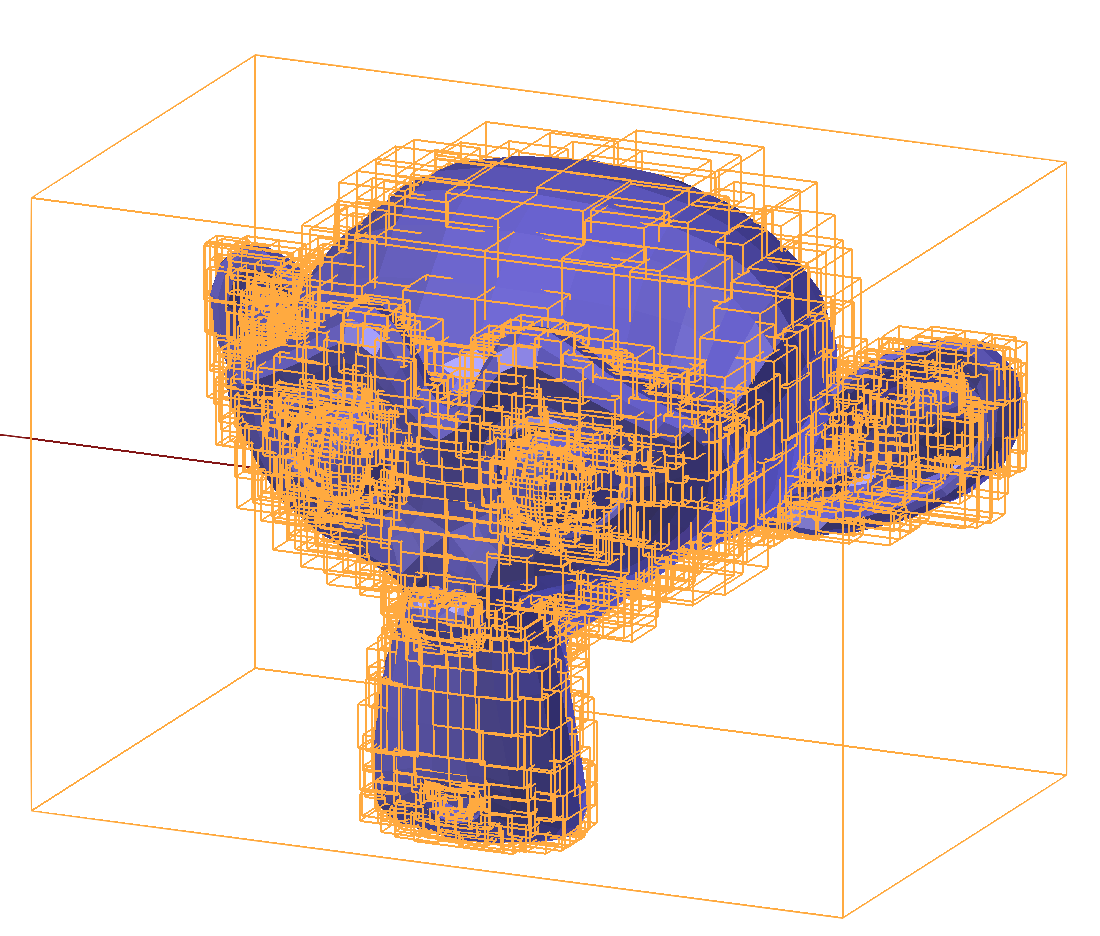
\includegraphics[width=0.5\linewidth]{octreeSuzanne}
		\caption{Binary tree leaves of an arbitrary mesh from \textit{Blender}.}
		\label{octreeSuzanne}
	%\label{octree}
\end{figure}

More precisely, we first initialize the ray-sorting considering a bounding box, containing all \textit{rays} and all elements. After the first median subdivision, we have to distribute \textit{rays} inside the two new boxes. This stage is done in $O(N)$ operations using W.Amy \textit{et al.} algorithm \cite{AABB}. Each box has $N_1$ and $N_2$ \textit{rays}, such as $N = N_1 + N_2$. Assuming this subdivision performed recursively to the $p$-level, each box contains $(N_i)$ \textit{rays} such as: 
\begin{equation}
N = \sum_{i=1}^{2^p} N_i.
\end{equation}  
Then, ray sorting at the $(p+1)$-level also conducts to $O(N)$ operations. To reach the leaves-level, we have to perform $O(N \log M)$ operations, where $\log M$ is close to the depth of the binary tree. At the end, as we have only one element per box, the ray-element intersection only needs $O(N)$ operations. Finally, instead of $O(N M)$ operations, we compute ray-tracing algorithm in~: 
\begin{equation}
O(M\log M) + O(N \log M) + O(N),
\end{equation}  
witch is quasi-linear and computationaly faster (see table \ref{tabComplexite} and fig. \ref{times}).  More over, if binary tree is precomputed, each iteration of ray-tracing stand for :
\begin{equation}
O(N \log M) + O(N).
\end{equation}.  
 


\begin{figure}[h]
\centering
	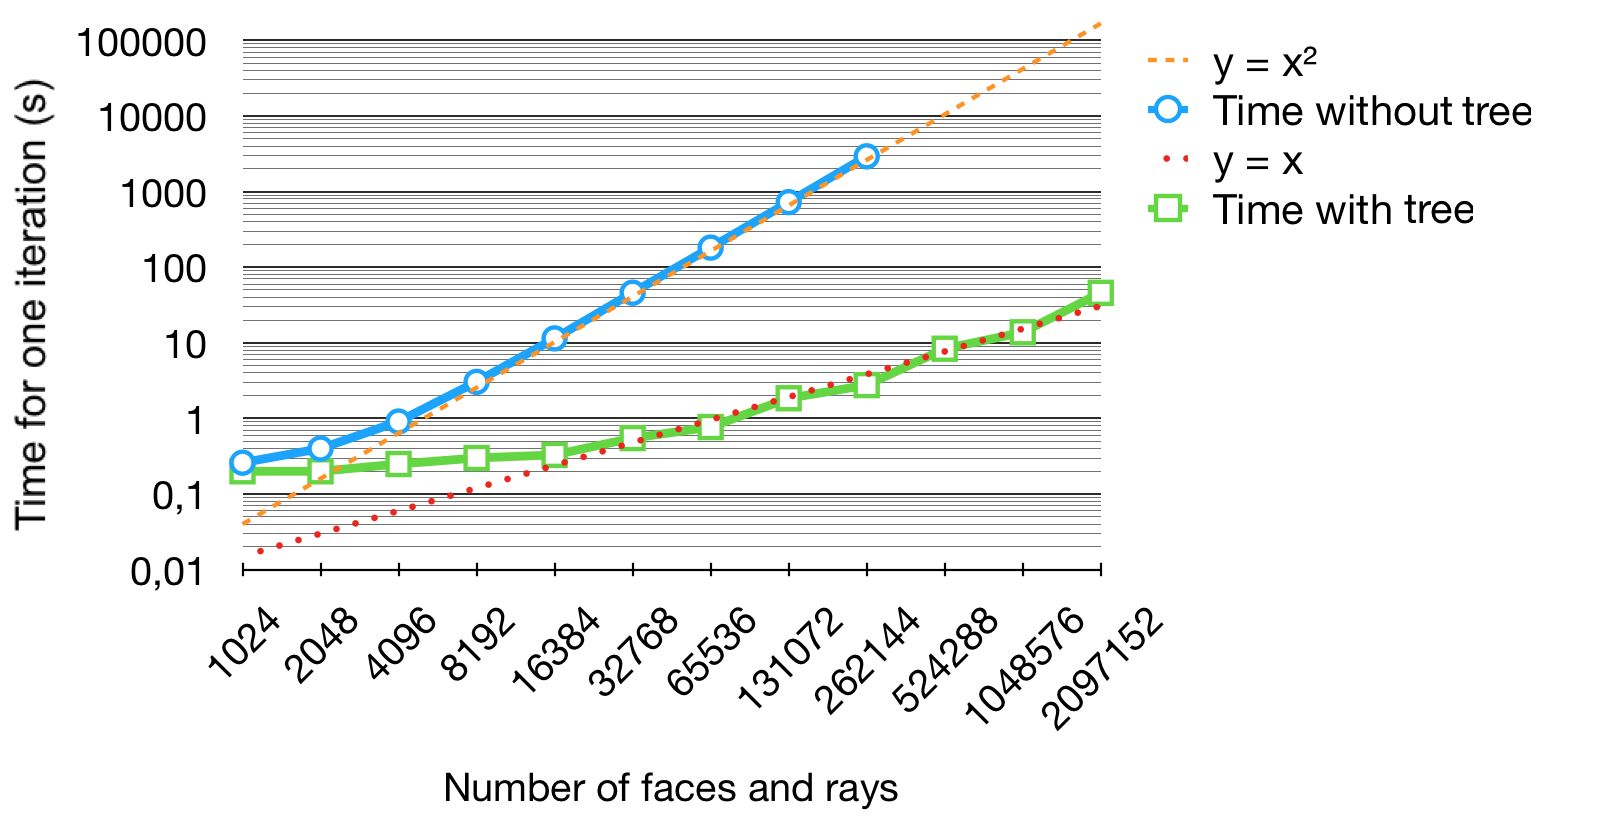
\includegraphics[width=0.8\linewidth]{times}
	\caption{Computation time for one iteration of ray-tracing in function of the number of face and rays, such as $N = M$ (log~scale). An omnidirectional source is located at the center of a mesh of a unitary tetrahedral.}
	\label{times}
\end{figure}
%
\begin{table}[h]
\centering
	\begin{tabular}{| c | c | c |}
		\hline
		Number of faces and \textit{rays} & Time \textbf{without} Octree (s) & Time \textbf{with} Octree (s)\\
		  \hline
		  \hline
		   $2^{10}$ (=1~024) & 0,26 &	0,2 \\
		   \hline
		$2^{11}$ (=2~048)  & 0,4	& 0,2 \\
		   \hline
		$2^{12}$ (=4~096) & 0,91	& 0,25\\
		   \hline
		$2^{13}$ (=8~192) & 3,05 &	0,3\\
		   \hline
		$2^{14}$ (=16~384) & 11,44	&0,33\\
		   \hline
		$2^{15}$ (=32~768) & 46,02	&0,55 \\
		     \hline
		    $2^{16}$ (=65~536) & 181,61	& 0,77\\
		   \hline
		$2^{17}$ (=131~072) & 725,17	& 1,85\\
		\hline
		$2^{18}$ (=262~144) & 2927,9 & 2,76 \\
		\hline
		$2^{19}$ (=524~288) & X & 8,36 \\
		\hline
		$2^{20}$ (=1~048~576) & X & 13,78 \\
		\hline
		%$2^{21}$ (=2~097~152) & X & 45,83 \\
		%\hline
	 \end{tabular}
	\caption{Computation time of fig. \ref{times}.}
	\label{tabComplexite}
\end{table}



\section{Numerical validation}
\subsection{Shoes box (modele complet)}
\subsection{Energy conservation (sphere reflechissante)}

\section{Application to Orange theater}

\section{Conclusion}

\subsection{Implementation}


To store the triangular faces in the box we test if the center of the face belongs to the box. Once each center has been store in the leaves of the octree (i.e the last boxes of the branches) we resize the leaves to embody the whole faces they contains. To test if a ray cross a box we use a pass/fail algorithm conceived for Axis-Aligned-Bounding-Box \cite{AABB}. This kind of box allow to simplify a lot the computation. 


We can can then measure the computation time of one iteration (i.e all \textit{rays} are intersecting a triangle) by increasing the number of \textit{rays} and the number of faces in the mesh. As we can see in the figure \ref{times} the complexity of the algorithm is almost linear by using the octree method. This allows to treat large meshes with millions of \textit{rays} by maintaining a low computation time. In particular, we can see in the table \ref{tabComplexite} that for 250~000 \textit{rays} and faces the computation time is divided by 1000 by using the octree. 


\newpage

\section{Validation}\label{sec5}

In order to validate our approach and our method we compare the experimental results with theoretical results. 

\subsection{Quadratic decrease}
First, to validate the quadratic decrease of the energy (see section \ref{sec2}) we observe the room impulse response of a cubic room whose all walls are 100\% absorbant except the walls on the x-axis (this may remind a Fabry-P\'erot interferometer). This particular room stands for a free space simulation where the distance between the source and the receiver is regularly increased. Furthermore, since the \textit{rays} spread on the x-axis and -x-axis and return in phase, the number of \textit{rays} received is twice the number of \textit{rays} in free space.
%
\begin{figure}[h]
\centering
	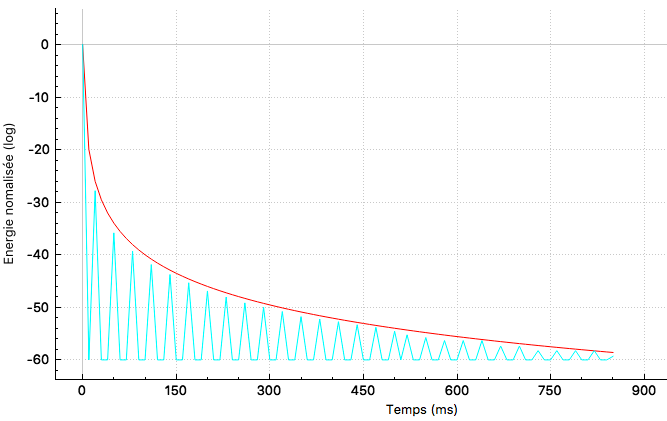
\includegraphics[width=0.6\linewidth]{test1}
	\caption{RIR in a Fabry-P\'erot-like configuration for 3 millions of \textit{rays} (blue) sampled at 100Hz and $f(x)=\frac{2}{x^2}$ (red)}
	\label{test1}
\end{figure}
%
The room impulse response (see fig. \ref{test1}) follows the function $f(x)=\frac{2}{x^2}$ which is the expected behavior. In free space, the number of \textit{rays} collected stands for the surfaces ratio and the quadratic decrease :
\begin{equation}
\frac{n}{N} = \frac{\int_s dS}{\int_{\sigma} dS} = \frac{\pi r^2}{4\pi d^2},
\end{equation}
with :
\begin{itemize}
\item$n$ : the number of \textit{rays} collected,
\item$N$ : the total number of \textit{rays},
\item$s$ : the constant surface of the receiver (disk) collecting \textit{rays},
\item$\sigma$ : the emission sphere surface,
\item$r$ : the constant radius of the receiver,
\item$d$ : the emission sphere radius (i.e the distance between the source and the receiver).
\end{itemize}

\subsection {Energy conservation}
The second test allows to simulate the conservation of the energy. We use a 100\% reflecting sphere (2m radius) pretty well refined (300~000 faces) and position the source and the receiver in the center. At each iteration all the \textit{rays} refocus in the center of the sphere and then are captured by the receiver.
\begin{figure}[h]
\centering
	\begin{subfigure}{0.45\textwidth}
		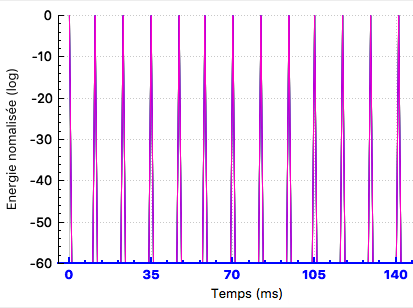
\includegraphics[width=\linewidth]{test2RIR}
		\caption{RIR for a 100\% reflecting sphere - 12 iterations}
		\label{test2RIR}
	\end{subfigure}
	\quad
	\begin{subfigure}{0.38\textwidth}
		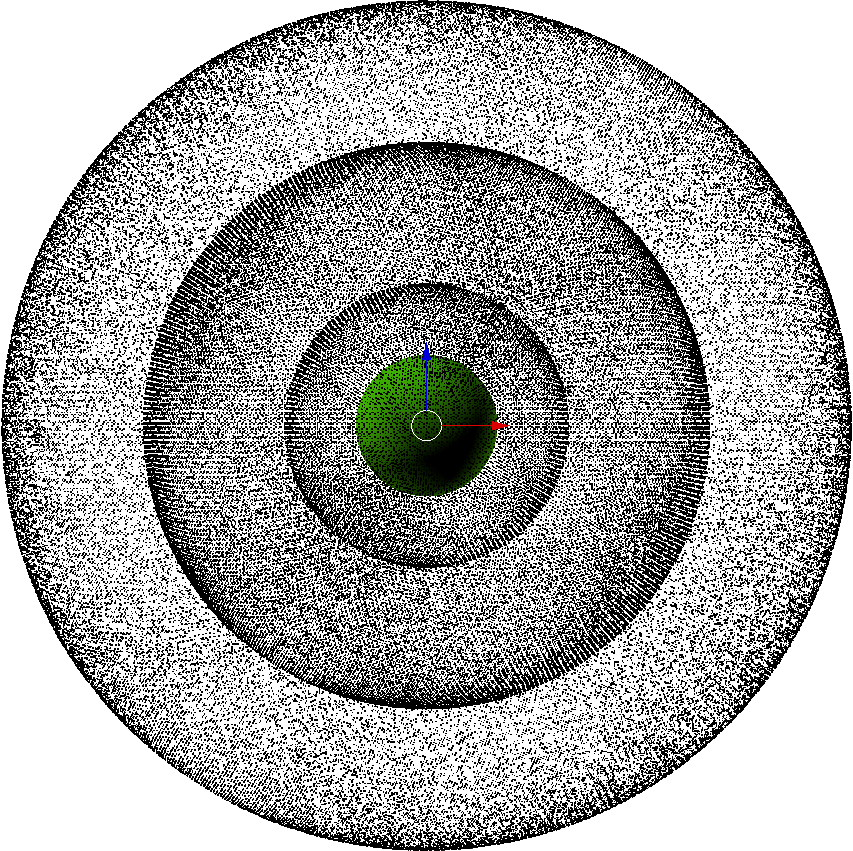
\includegraphics[width=\linewidth]{test2SI}
		\caption{Position of the images-sources - 4 iterations}
		\label{test2SI}
	\end{subfigure}
	\caption{100\% reflecting sphere}
\end{figure}
%
We observe the expected result as the room impulse response is a Dirac comb (see fig. \ref{test2RIR}) and the image-sources are positioned on spheres whose radius doubles at each iteration (see fig. \ref{test2SI}).
%
\begin{figure}[h]
\centering
	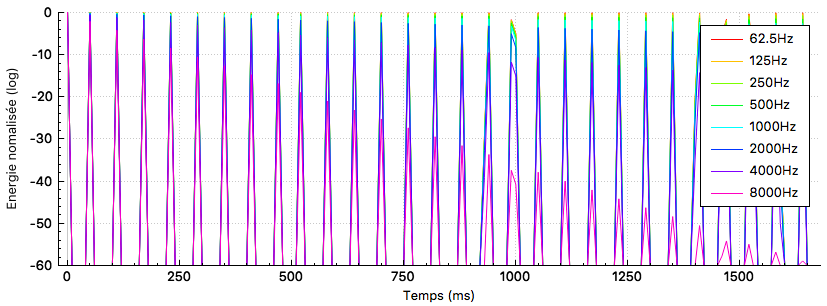
\includegraphics[width=0.6\linewidth]{test2absair}
	\caption{RIR for a 100\% reflecting sphere with air absorption - 30 iterations}
	\label{test2absair}
\end{figure}
%
By adding the air absorption (see fig. \ref{test2absair}) we can observe that the highest frequencies decrease faster than the lowest which reflect the nature behavior.

\subsection{Shoe box case}
To finalize the validation algorithm we compare the results of a shoe box type room with an analytic computation. The image-sources can be positioned in space with the following formula \cite{mcgovern} :
\begin{align}
P_{is} = i \times D + P_s \times (-1)^i,
\end{align}
with : 
\begin{itemize}
\item$i \in (-n, n)$ and $n \in \mathbb{N}$,
\item$P_{is}$ : the image-source position coordinate on X, Y or Z,
\item$P_s$ : the source position coordinate on X, Y or Z,
\item$D$ : the room dimension on X, Y or Z.
\end{itemize}
The energy of each image-source is $\frac{1}{d^2}$ where $d$ is the distance between the image-source avec the receiver. If we compare the position of these theoretical image-sources with the image-sources obtained with the algorithm, we get the exact same result to the float precision ($10^{-6}m$). Concerning the energy, we compare two kind of errors : the relative error such as :
\begin{align}
\epsilon_{rel} = \frac{|E_{exp}-E_{theo}|}{E_{theo}},
\end{align}
and the infinity norm error which express the fact that the further away the image-source is from the receiver, the less important the error will be for the final result.
\begin{align}
\epsilon_{\infty} = \frac{|E_{exp}-E_{theo}|}{\max(E_{theo})}.
\end{align}
We can also add some absorption coefficient on the walls and take into account the air absorption. We can see in the figure \ref{test3_8} that the relative error of the energy image-source per image-source remains always below 5\%. In the same way we see in the figure \ref{test3_9} that the infinity norm error is below $0,3\%$ for all frequencies.

\begin{figure}[h]
\centering
	\begin{subfigure}{0.49\textwidth}
		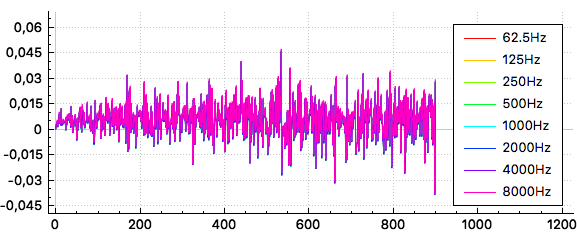
\includegraphics[width=\linewidth]{test3_8}
		\caption{Relative error}
		\label{test3_8}
	\end{subfigure}
	\begin{subfigure}{0.49\textwidth}
		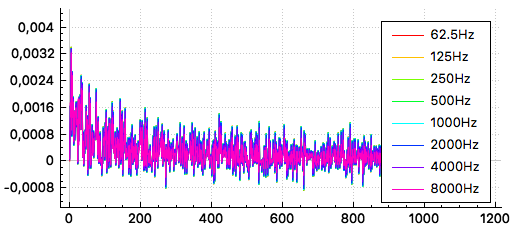
\includegraphics[width=\linewidth]{test3_9}
		\caption{Infinity norm error}
		\label{test3_9}
	\end{subfigure}
	\caption{Error for each image-sources with walls and air absorption - 1~000~000 \textit{rays}}
\end{figure}


\newpage

\section{Developed softwares }\label{sec6}

The room acoustic tool is available in two forms. 

\subsection{Matlab library}
First a Matlab library \cite{gypsilab} ... \\

\subsection{Blender add-on}
In a second hand the tool is also available as a Blender add-on. The user can work on the CAD software to model the room under test, positioning the sources and the receiver and assign materials to the walls. By clicking on the "Run" button, the mesh is exported, the materials are linked to eight absorption coefficients (extracted from a data base) and the acoustic calculation tool is launched. This is an executable C++ complied software which treats information form Blender and generates the room impulse response. The communication between the CAD and the executable is done thanks to an .obj file, so using Blender is not necessary. Different options allow to analyse the results by reimporting \textit{rays} or image-sources on the CAD software. It is also possible to listen an audio file convolved to the RIR to listen the reverberate sound.


%\begin{figure}
%	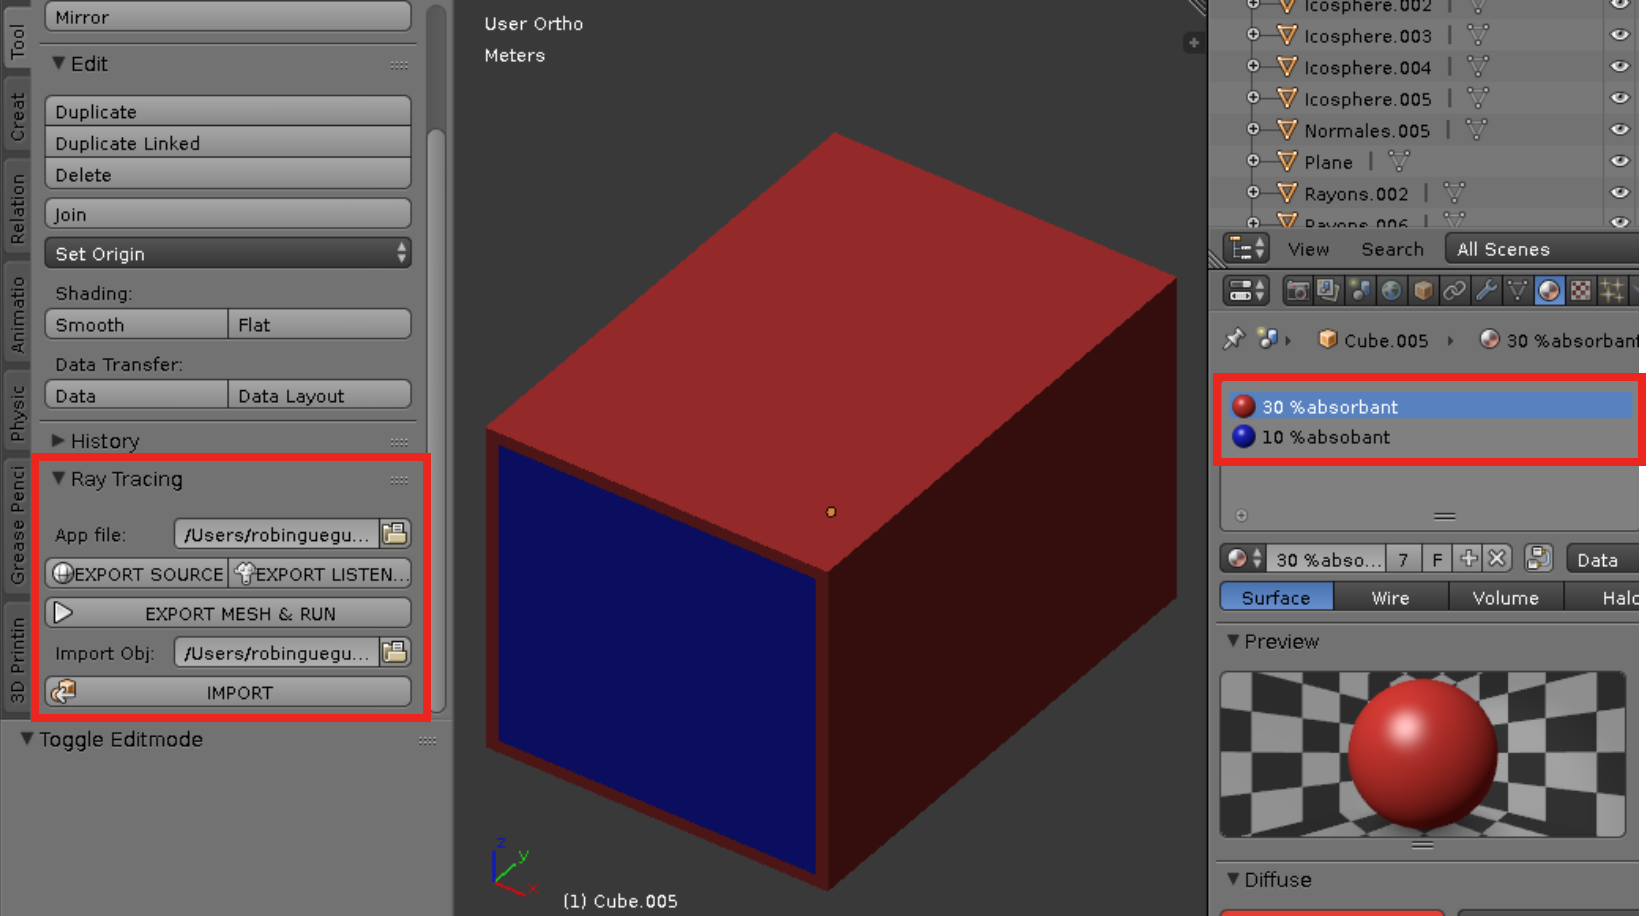
\includegraphics[width=\linewidth]{add-on}
%	\caption{Add-on Blender}
%\end{figure}

\begin{figure}[h]
\centering
	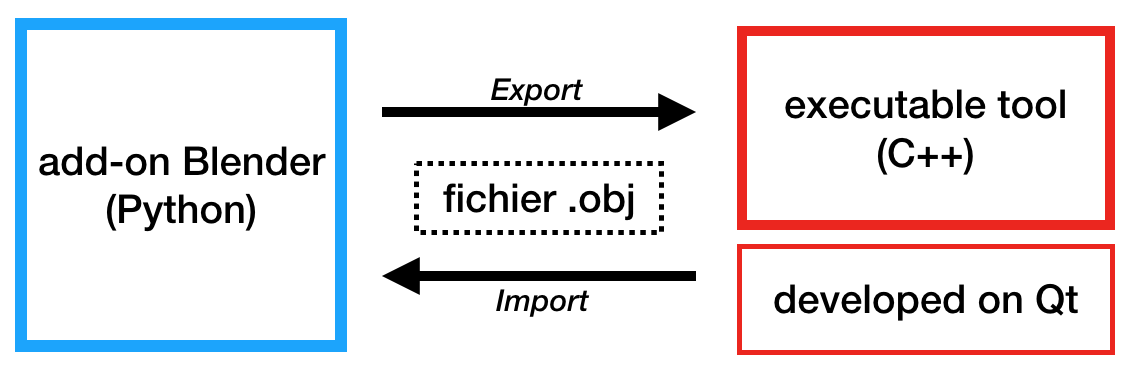
\includegraphics[width=0.5\linewidth]{software}
	\caption{Software architecture}
\end{figure}

\begin{figure}[h]
\centering
	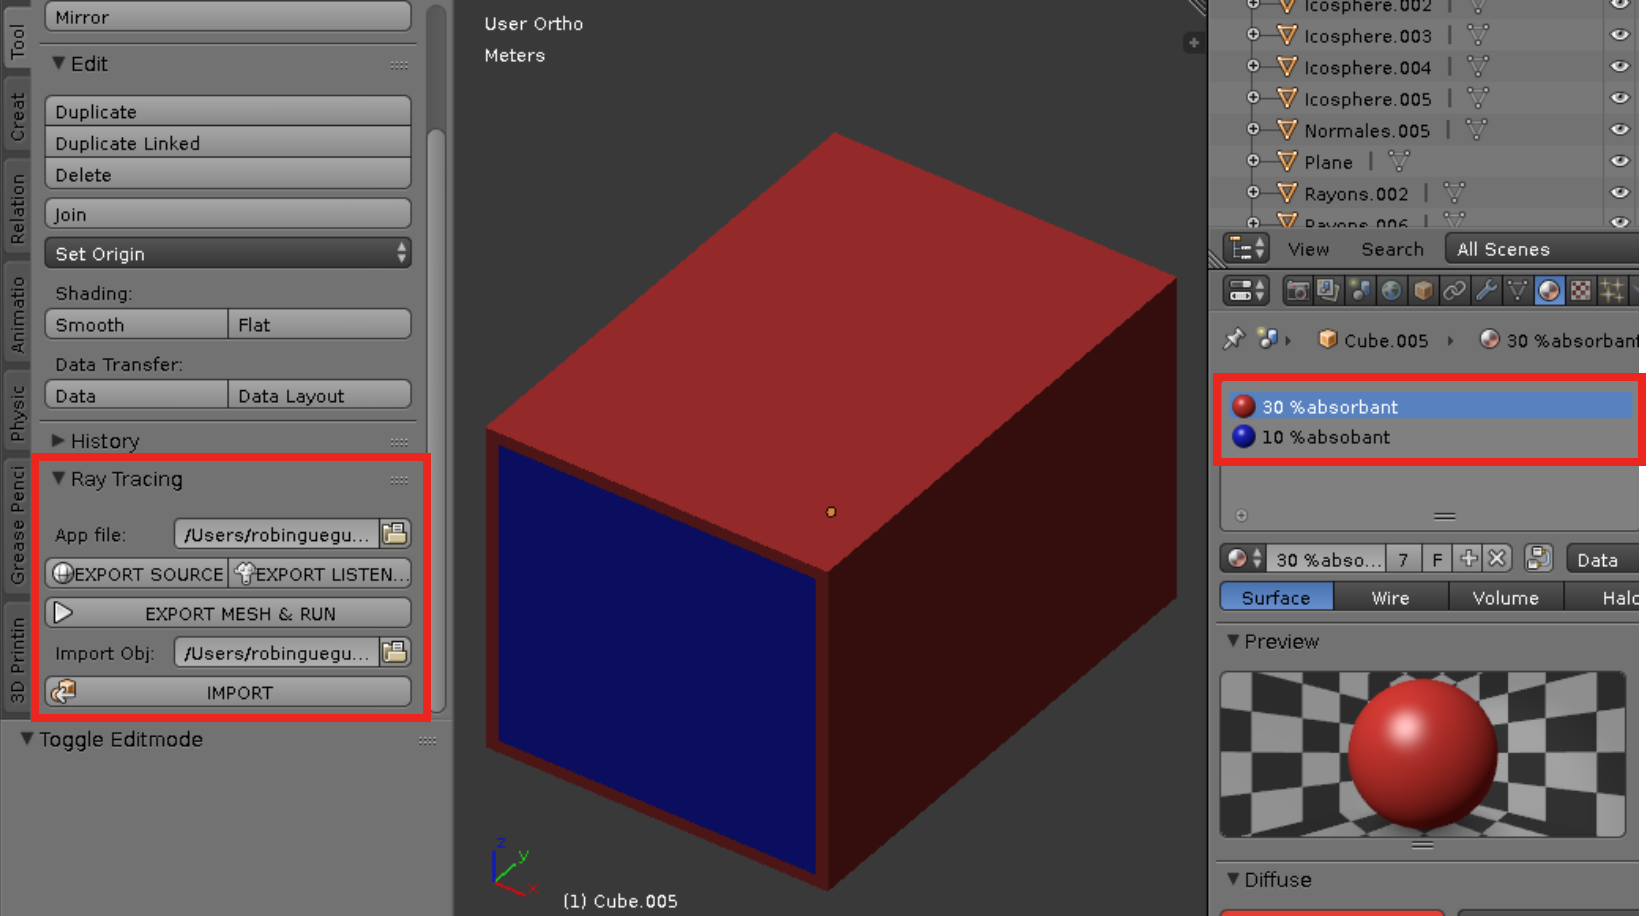
\includegraphics[width=0.8\linewidth]{add-on}
	\caption{Add-on Blender for exporting/importing meshes and running computation tool}
	\label{add-on}
\end{figure}


\section{Application to the antic theatre of Orange}\label{sec7}

\begin{figure}[h]
\centering
	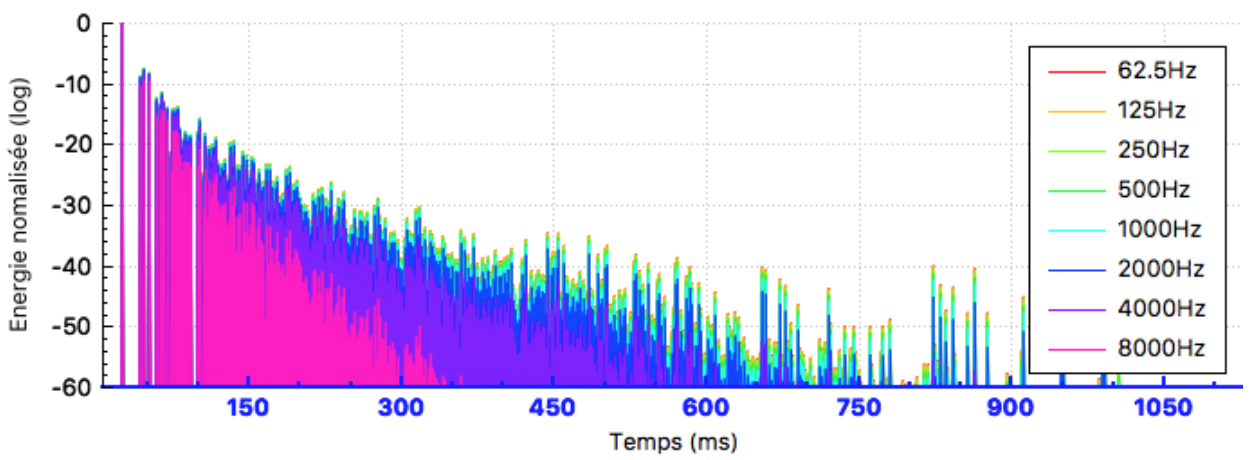
\includegraphics[width=0.7\linewidth]{rir}
	\caption{Room impulse response of the antic theater of Orange}
	\label{rir}
\end{figure}

The acoustic simulation can be done on the ancient theater of Orange. Because it is an open room the software automatically add a 100\% absorbant box around the building to be sure to always count all \textit{rays}. We can then calculate the image-sources and the RIR for different configurations of the theatre or different materials. Indeed, archeologists want to explore some architecture hypothesis from missing part of the theatre. An acoustical analysis can allow to understand some behaviors like : the influence of the position of the spectators in the bleachers, the shape of the roof, the materials of the \textit{orchestra}, etc. With a 600~000 faces theatre (i.e including decoration elements of the stage wall), the RIR at $RT_{60}$ is generated in 20 minutes for one million \textit{rays} (see fig. \ref{rir}). Each iteration is done in 25s so it really depends on the materials chosen. We can note that the more details of the mesh are refined the more we can simulate diffraction effect. Indeed, in high frequency, small detail elements will be able to reflect the \textit{rays} in different directions which can resemble diffraction effects. In the theater it will be really interesting to study where the reflection come from. Thus, we project the image-sources on the wall of the theater to understand what wall is the main contributor to the energy received (see fig. \ref{theatre}).

\begin{figure}[h]
\centering
	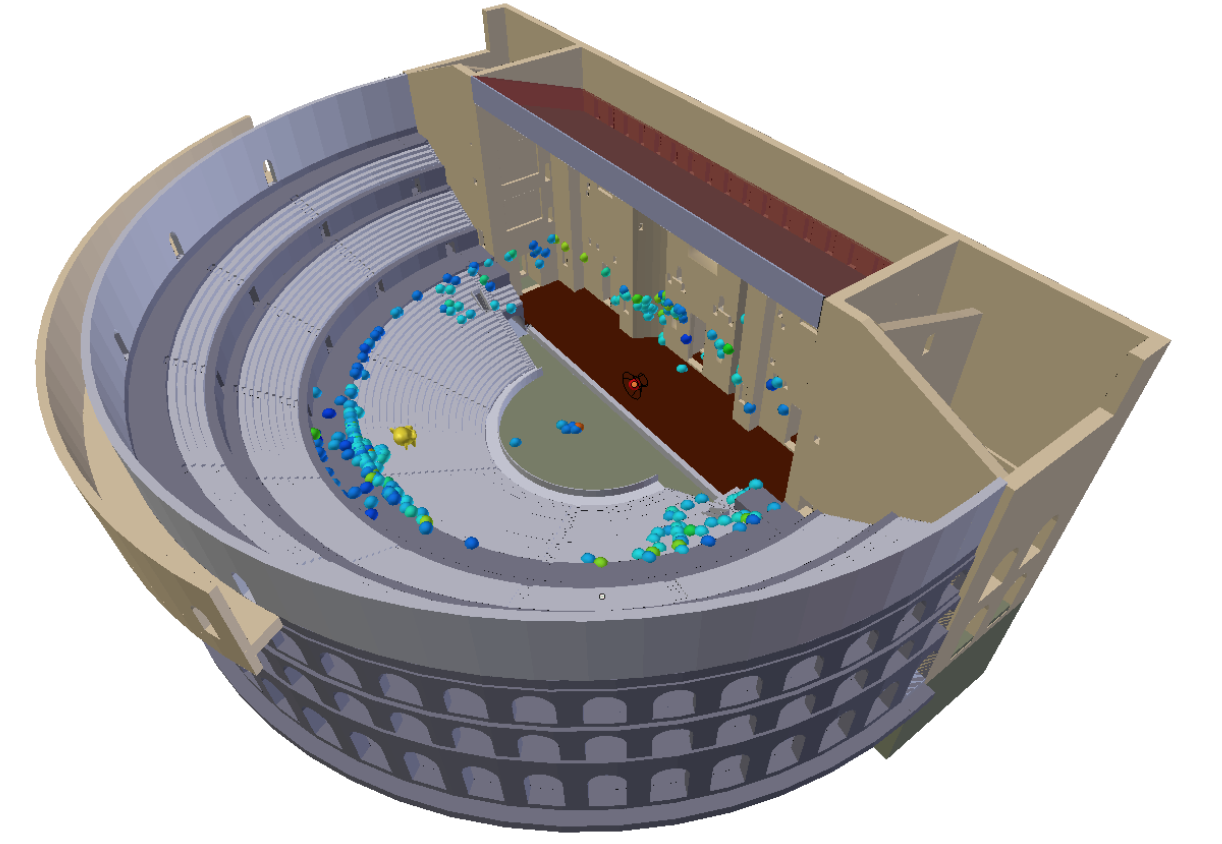
\includegraphics[width=0.7\linewidth]{theatre}
	\caption{Images-sources projected on the theatre of Orange}
	\label{theatre}
\end{figure}


\section{Conclusions}

We presented the problems raised by an acoustic study of an ancient monument. The complex geometry of this type of building and their colossal size requires the use of approximate calculation methods. Thus, by simulating the reflections and absorptions of the walls, it is possible to study the reverberation of a room. Despite the inevitable approximations of the model, we have proved that the laws of physics are respected. A fast algorithm has been implemented to allow users to easily and quickly test their architectural assumptions. Thus, the calculation time becomes linear to the product number of mesh elements/number of \textit{rays}. The algorithm developed allows the study of the temporal graph of reverberation of the building as well as the position in space of the various sound reflections. Furthermore, a sound signal could be heard in three dimensions thanks to binaural filters and steering control can be done with "Head Tracker" mounted on a headset.

However, there are many opportunities for improvement that remain under consideration for this type of software tool. First, in a context where virtual reality is becoming more and more important in today's applications, we could consider moving the listener in real time and thus, allow a complete virtual tour of the building. Secondly, from the point of view of the analysis results, there are many possible improvements at the graphic level. That raises some questions. How to view acoustic calculation results? What information is essential for an archaeologist wishing to study the acoustics of a monument? Similarly, is it essential to add diffraction effects to the model? If so, what is the best method? Could certain acoustic behaviours be treated locally and then inserted into the model by ray tracing? Finally, it would also be interesting to use sources whose directivity is not uniform. This would be more representative of the real cases, and in particular, of the use made in Orange at the theatre origin. The sounds were then emitted by musical instruments or by the human voice possibly amplified by a mask.



\section*{Acknowledgments}
The authors would particularly like to thank Fran\c{c}ois Alouges, Titien Bartet, Pascal Frey and Emmanuelle Rosso for all the help they each provided at the different stages of this project. Thanks also to Jean-Dominique Polack for his wise advice on architectural acoustics.

%\subsection*{Author contributions}
 

%\subsection*{Financial disclosure}


%\subsection*{Conflict of interest}



%\section*{Supporting information}

%The following supporting information is available as part of the online article:
%
%\noindent
%\textbf{Figure S1.}
%{500{\uns}hPa geopotential anomalies for GC2C calculated against the ERA Interim reanalysis. The period is 1989--2008.}
%
%\noindent
%\textbf{Figure S2.}
%{The SST anomalies for GC2C calculated against the observations (OIsst).}


%\section{Glossary\label{app1}}

%\printglossaries


	

	
		
%Use \verb+\begin{verbatim}...\end{verbatim}+ for program codes without math. Use \verb+\begin{alltt}...\end{alltt}+ for program codes with math. Based on the text provided inside the optional argument of \verb+\begin{code}[Psecode|Listing|Box|Code|+\hfill\break \verb+Specification|Procedure|Sourcecode|Program]...+ \verb+\end{code}+ tag corresponding boxed like floats are generated. Also note that \verb+\begin{code}[Code|Listing]...+ \verb+\end{code}+ tag with either Code or Listing text as optional argument text are set with computer modern typewriter font.  All other code environments are set with normal text font. Refer below example:
%
%\begin{lstlisting}[caption={Descriptive Caption Text},label=DescriptiveLabel]
%for i:=maxint to 0 do
%begin
%{ do nothing }
%end;
%Write('Case insensitive ');
%WritE('Pascal keywords.');
%\end{lstlisting}
%
%
%
%\subsection{Subsection title of first appendix\label{app1.1a}}
%
%\noindent\textbf{Unnumbered figure}
%
%
%\begin{center}
%
\includegraphics[width=7pc,height=8pc,draft]{empty}
%\end{center}
%
%
%%== Figure 4 ==
%%% Example for figure inside appendix
%\begin{figure}[t]
%\centerline{
\includegraphics[height=10pc,width=78mm,draft]{empty}}
%\caption{This is an example for appendix figure.\label{fig5}}
%\end{figure}


%\nocite{*}% Show all bib entries - both cited and uncited; comment this line to view only cited bib entries;
\bibliography{Biblio}%

\clearpage

%\section*{Author Biography}

%\begin{biography}{
\includegraphics[width=66pt,height=86pt,draft]{empty}}{\textbf{Author Name.} This is sample author biography text this is sample author biography text this is sample author biography text this is sample author biography text this is sample author biography text this is sample author biography text this is sample author biography text this is sample author biography text this is sample author biography text this is sample author biography text this is sample author biography text this is sample author biography text this is sample author biography text this is sample author biography text this is sample author biography text this is sample author biography text this is sample author biography text this is sample author biography text this is sample author biography text this is sample author biography text this is sample author biography text.}
%\end{biography}

\end{document}
